\chapter{Nástroj pro analýzu kontraktů}
	Cílem práce z hlediska implementace bylo vytvořit nástroj, který by umožňoval získání dat podle výše navrženého modelu ze zdrojové či přeložené formy Java programu. Výsledná aplikace by pak měla umožnit vytvoření externí reprezentace dat a případně také porovnání DbC konstrukcí. Nástroj by měl být schopen zpracovat alespoň dva způsoby popisu DbC konstrukcí a měl by dovolovat snadné rozšíření pro další způsoby. S využitím tohoto nástroje by pak měla být vytvořena jednoduchá uživatelská aplikace, která by sloužila k načtení a zobrazení dat modelu.\\
	
	Smyslem aplikace je umožnit detekci kontraktů ve zdrojových, respektive přeložených, souborech jazyka Java. Nalezené kontrakty je pak možné analyzovat a zkoumat způsob a četnost použití jednotlivých typů v různých projektech. Aby bylo možno získaná data dále analyzovat, je zde také export do formátu JSON. Nástroj umožňuje porovnání dvou adresářů se soubory, což může být užitečné zejména při porovnání různých verzí projektu. Můžeme tak zjistit, zda se nezměnilo rozhraní či zda se zpřísnily podmínky kontraktů oproti předchozí verzi.\\
	
	Celý nástroj je rozdělen do dvou velkých částí. První z nich je knihovna, která poskytuje všechny potřebné metody pro práci se soubory jazyka Java, jejich analýzu a zpracování, extrakci kontraktů a jejich následné porovnání a export. Druhou částí je uživatelská aplikace, která využívá metod této knihovny a umožňuje její pohodlnou obsluhu. Tento vztah je znázorněn na stručném obrázku \ref{globalArchitecture}. Na obrázku \ref{componentDiagram} je pak vidět komponentový diagram, který obsahuje více podrobností.
					
	\begin{figure}[!htb]
		\minipage{1\textwidth}	
			\centering
			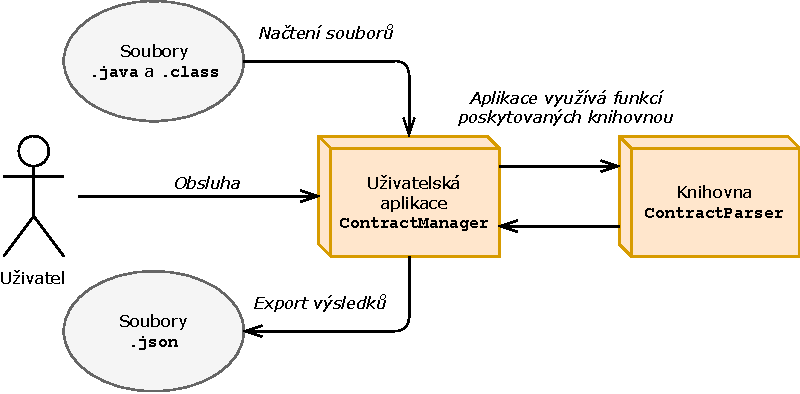
\includegraphics{img/globalArchitecture.pdf}
			\caption[globalArchitecture]{Architektura nástroje}
			\label{globalArchitecture}
		\endminipage\hfill
	\end{figure}
	
	\begin{figure}[!htb]
		\minipage{1\textwidth}	
			\centering
			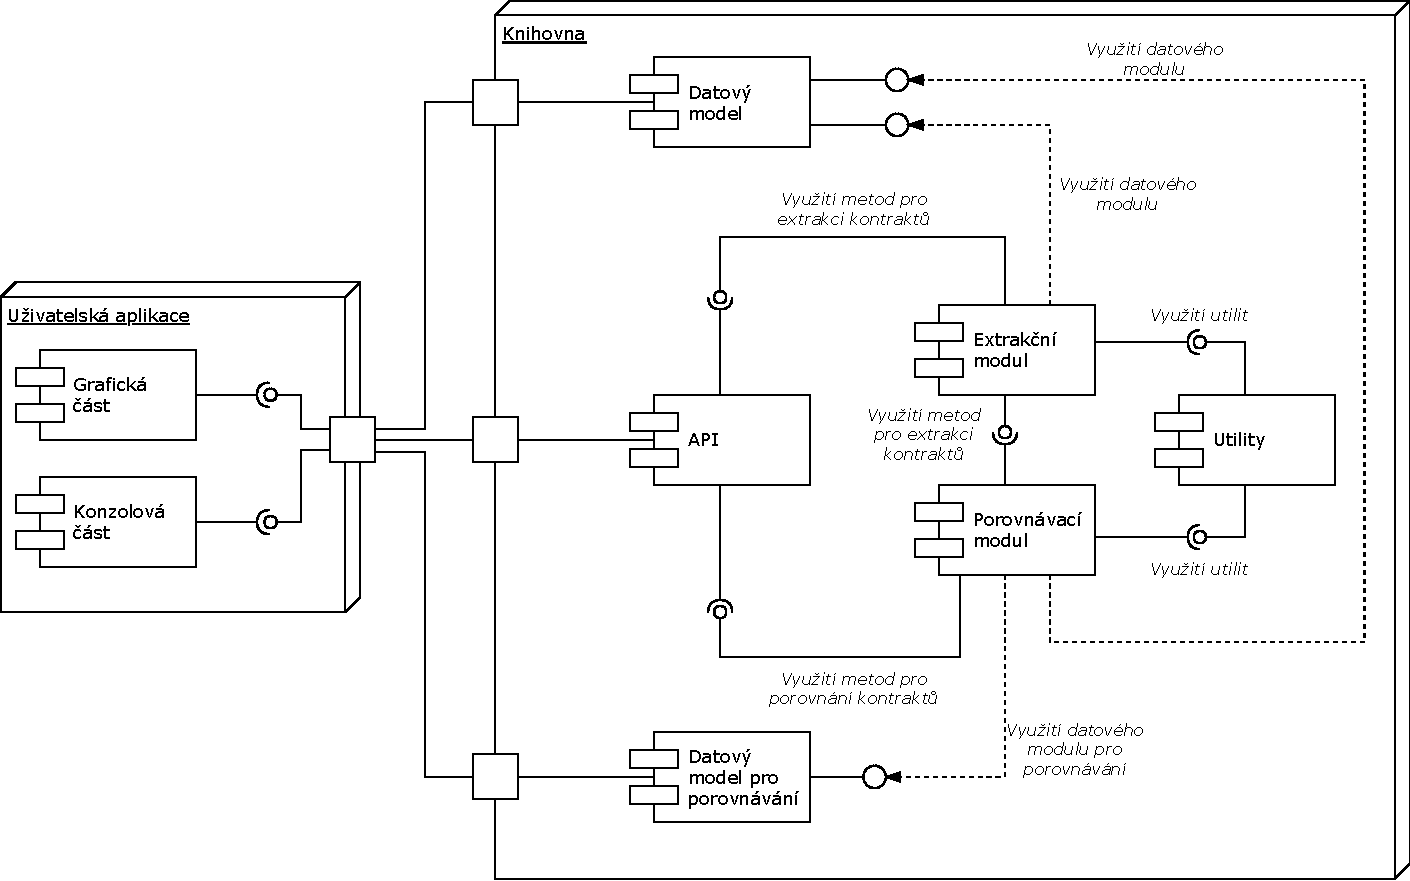
\includegraphics[width=1\textwidth]{img/componentDiagram.pdf}
			\caption[componentDiagram]{Komponentový diagram nástroje}
			\label{componentDiagram}
		\endminipage\hfill
	\end{figure}		
	
	% struktura projektu a potom v textu důležité třídy v implementaci + možná jejich uml model
	
%%%%%%%%%%%%%%%%%%%%%%%%%%%%%%%%%%%%%%%%%%%%%%%%%%%%%%%%%%%%%%%%%%%%%%%%%%%%%%%%%%%%%%%%%%%%%%%%%%%%%%%%%%%%%%%%%%%%%%%%%%%%%%%%%%%%%%%%%%%%%%%%%%%%%%%%%%%%%%%%%%%%%%%%%%%%%%%%%%%%%%%%
%%%%%%%%%%%%%%%%%%%%%%%%%%%%%%%%%%%%%%%%%%%%%%%%%%%%%%%%%%%%%%%%%%%%%%%%%%%%%%%%%%%%%%%%%%%%%%%%%%%%%%%%%%%%%%%%%%%%%%%%%%%%%%%%%%%%%%%%%%%%%%%%%%%%%%%%%%%%%%%%%%%%%%%%%%%%%%%%%%%%%%%%
%%%%%%%%%%%%%%%%%%%%%%%%%%%%%%%%%%%%%%%%%%%%%%%%%%%%%%%%%%%%%%%%%%%%%%%%%%%%%%%%%%%%%%%%%%%%%%%%%%%%%%%%%%%%%%%%%%%%%%%%%%%%%%%%%%%%%%%%%%%%%%%%%%%%%%%%%%%%%%%%%%%%%%%%%%%%%%%%%%%%%%%%
%%%%%%%%%%%%%%%%%%%%%%%%%%%%%%%%%%%%%%%%%%%%%%%%%%%%%%%%%%%%%%%%%%%%%%%%%%%%%%%%%%%%%%%%%%%%%%%%%%%%%%%%%%%%%%%%%%%%%%%%%%%%%%%%%%%%%%%%%%%%%%%%%%%%%%%%%%%%%%%%%%%%%%%%%%%%%%%%%%%%%%%%
	\section{Knihovna}
		Pro realizace nástroje jsem se rozhodl implementovat knihovnu, která poskytuje metody potřebné pro extrakci, porovnání a export kontraktů. Její součástí je také samozřejmě model použitý pro jejich reprezentaci. 

%%%%%%%%%%%%%%%%%%%%%%%%%%%%%%%%%%%%%%%%%%%%%%%%%%%%%%%%%%%%%%%%%%%%%%%%%%%%%%%%%%%%%%%%%%%%%%%%%%%%%%%%%%%%%%%%%%%%%%%%%%%%%%%%%%%%%%%%%%%%%%%%%%%%%%%%%%%%%%%%%%%%%%%%%%%%%%%%%%%%%%%%	
	    \subsection{Použité technologie}
	    
	    	\subsubsection{Programovací jazyk}
				Pro realizaci knihovny jsem použil jazyk Java verze 1.8. Jedním z hlavních důvodů bylo, že nástroj zkoumá reprezentace kontraktů v jazyce Java, díky tomu je možné dané konstrukce snadno testovat a zkoušet přímo v tomto projektu. Vedoucí práce také upřednostňoval použití jazyka Java z důvodů případného propojení s jinými nástroji, které byly vyvinuty pro práci s kontrakty v rámci univerzity a jsou také realizovány v Java. Osobně mám s jazykem Java pravděpodobně největší zkušenosti, což byl další z důvodů, proč tento jazyk použít. Z těchto důvodů byla volba jazyka poměrně jednoznačná.\\
				
				I přesto, že v průběhu vývoje projektu vyšla verze Java 1.9 a posléze i 1.10, rozhodl jsem se po domluvě s vedoucím práce ponechat stabilní verzi 1.8 a nepřecházet v průběhu vývoje na novější verzi jazyka.
				
			\subsubsection{Vývojové prostředí}				
				Nástroj byl realizován ve vývojovém prostředí IDEA IntelliJ Ultimate 2017.3.3.
	    	
			\subsubsection{Práce se závislostmi}
				Pro zajištění závislostí jako jsou knihovny třetích stran, ale také pro snadnou distribuci knihovny jsem zvolil technologii Apache Maven \cite{maven}. Jedná se o široce používaný nástroj pro získávání závislostí a tvorbu projektů.
				
			\subsubsection{Logování}
				Pro logování, tedy zobrazení a uložení chybových či informačních zpráv, byla použita knihovna Apache Log4j \cite{log4j}. Tato knihovna umožňuje pokročilé možnosti logování, které je možné dobře nastavit pomocí konfiguračních souborů. Opět se jedná o široce používanou technologii.
				
			\subsubsection{Tokenizace zdrojových souborů jazyka Java}
				Pro implementaci tokenizace souborů jsem se rozhodl použít knihovnu JavaParser \cite{javaparser}. Učinil jsem tak na základě mého průzkumu (viz 4. kapitola Tokenizace jazyka Java). Knihovna poskytuje komplexní reprezentaci daného zdrojového souboru a je tak možné jej dále analyzovat a zpracovávat. Knihovnu je možné snadno použít přímo v projektu díky zprostředkovanému API.
			
			\subsubsection{Dekompilace přeložených souborů jazyka Java}
				Jako dekompilátor přeložených souborů jazyka Java (\texttt{.class}) jsem použil knihovnu Procyon \cite{procyon}. Jedná se o nástroj, který umožňuje snadnou dekompilaci souborů a to včetně moderních konstrukcí jazyka Java. Hlavním důvodem volby této knihovny byla možnost použití dekompilace v rámci kódu za pomocí API.
				
			\subsubsection{Práce s formátem JSON}
				Pro ukládání reprezentací do formátu JSON byla použita knihovna Gson \cite{gson}. Umožňuje intuitivní převod objektu typu Java\footnote{Mohou použity téměř libovolné objekty, avšak nesmějí být cyklické (Objekt nesmí ve své hierarchii atributů opět obsahovat tentýž objekt)} do formátu JSON za pomocí API. Mimo jiné také umožňuje formátování \emph{Pretty Print}, které je lépe čitelné pro člověka.
				
			\subsubsection{Testování}
				Pro tvorbu jednotkových testů byla použita technologie jUnit 5 \cite{junit}.   	 


%%%%%%%%%%%%%%%%%%%%%%%%%%%%%%%%%%%%%%%%%%%%%%%%%%%%%%%%%%%%%%%%%%%%%%%%%%%%%%%%%%%%%%%%%%%%%%%%%%%%%%%%%%%%%%%%%%%%%%%%%%%%%%%%%%%%%%%%%%%%%%%%%%%%%%%%%%%%%%%%%%%%%%%%%%%%%%%%%%%%%%%%	

		\subsection{Návrh nástroje}
			Celý nástroj je rozdělen do několika modulů, viz obrázek \ref{componentDiagram}. Oba datové modely byly popsaný výše v 5. kapitole - Datový model. Parsovací modul je klíčovou součástí celého nástroje. Umožňuje zpracování kódu jazyka Java a jeho analýzu. Poskytuje prostředky pro uležení tohoto analyzovaného kódu do navržené struktury a následnou extrakci kontraktů. Porovnávací modul umožňuje porovnávání složek a souborů z hlediska kontraktů a API. Utility poskytují metody pro práci se zdroji, soubory. API je navržena pro snadné vnější použití celé knihovny. Jednotlivé moduly jsou popsány níže.		
		
				\begin{figure}[!htb]
					\minipage{1\textwidth}	
						\centering
						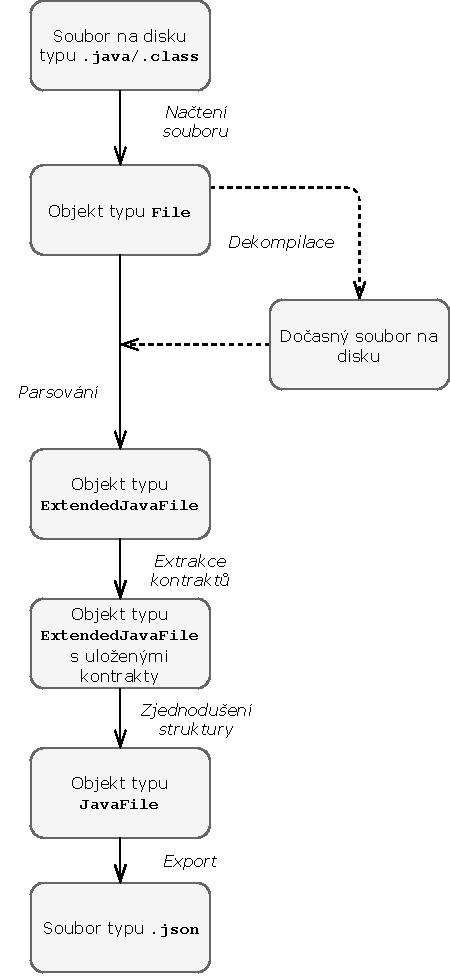
\includegraphics{img/workFlow.pdf}
						\caption[workFlow]{Základní work flow}
						\label{workFlow}
					\endminipage\hfill
				\end{figure}
				
				
%%%%%%%%%%%%%%%%%%%%%%%%%%%%%%%%%%%%%%%%%%%%%%%%%%%%%%%%%%%%%%%%%%%%%%%%%%%%%%%%%%%%%%%%%%%%%%%%%%%%%%%%%%%%%%%%%%%%%%%%%%%%%%%%%%%%%%%%%%%%%%%%%%%%%%%%%%%%%%%%%%%%%%%%%%%%%%%%%%%%%%%%

		\subsection{Parsovací modul}
			Tento modul zajišťuje zpracování zdrojových souborů jazyka Java a následné uložení do reprezentace \texttt{ExtendedJavaFile}. To má na starosti třída \texttt{JavaFileParser}, která také využívá třídy \texttt{MethodVisitor}.\\
			
			Třída \texttt{ExtendedJavaFile} je součástí modelu pro parsování, který dědí od svých rodičovských tříd ze základního datového modelu výše. Dále je zde třída \texttt{ExtendedJavaClass} a \texttt{ExtendedJavaMethod}. Tento rozšířený model ukládá dodatečné informace jako je tělo metod, anotace atd. Z těchto informací jsou následně získávány kontrakty.\\
			
			Vytvořená struktura je následně procházena a jsou z ní extrahovány kontrakty. To zajišťují třídy \texttt{GuavaParser} a \texttt{JSR305Parser} (každá svůj cílený typ kontraktu). Tyto třídy implementují rozhraní \texttt{ContractParser} a továrna \texttt{ParserFactory} umožňuje vytváření jejich instancí. Tímto způsobem se instance objektu \texttt{ExtendedJavaFile} postupně rozšiřuje.\\
			
			Poté co byly extrahovány všechny kontrakty, podrobnosti o metodách a třídách jsou již redundantní a z toho důvodu je objekt \texttt{ExtendedJavaFile} zredukován na \texttt{JavaFile}. Totéž platí pro zbytek modelu. K této redukci slouží třída \texttt{Simplifier}.\\
			
			Poslední částí tohoto modulu je třída \texttt{ContractExtractor}. Ta slouží jako výchozí bod pro komunikaci s ostatními částmi nástroje a spojuje dílčí třídy a jejich funkce dohromady. V podstatě se jedná o API pro vnitřní užití knihovny.\\
			
			Graficky je možné vidět tento modul v podobě UML diagramu, který je zobrazen na obrázku \ref{UMLParser}. Jedná se o zjednodušený UML diagram tříd, kde jsou jednotlivé metody omezeny pouze na svůj název a návratovou hodnotu. Důvodem je to, že metody mají mnoho vstupních parametrů, což by činilo diagram nepřehledný. Podrobnosti o konkrétních třídách je pak možné získat z JavaDoc dokumentace(na CD ve složce \texttt{javaDoc}. Rozšíření model je také zjednodušen a jsou zde zobrazeny pouze atributy, které nemají rodičovské třídy zobrazené v modelu výše.
		
			\subsubsection{Parsování Java souborů}	    
				Pro zpracování zdrojových souborů jazyku Java byla použita knihovna JavaParser. Ta poskytuje metodu \texttt{parse()}, která vytvoří komplexní strukturu daného zdrojového souboru. V prvním kroku se tato struktura projde a vyhledá všechny třídy (\emph{class}) a také rozhraní \emph{interface} a výčtové typy \emph{enum}. Pro účely modelu jsou si tyto tři prvky rovny. Každý nalezený prvek je následně uložen do modelu. V případě třídy a rozhraní se struktura prochází dále a do modelu jsou uloženy všechny konstruktory, které se z hlediska modelu považují za metody (viz níže). Následně jsou uloženy všechny anotace dané \uv{třídy}.\\
			
				Po této přípravě je využita třída \texttt{MethodVisitor}, která dědí od třídy \texttt{VoidVisitorAdapter} a umožňuje procházet všechny metody v daném souboru. V metodě pak máme k dispozici objekt typu \texttt{MethodDeclaration}, který obsahuje všechny potřebné údaje a také rodičovský \texttt{ExtendedJavaFile}. Pro každou metodu je nalezena její rodičovská třída. Hledá se nejvyšší rodič a tudíž vnořené metody nemají jako rodiče vyšší metodu ale nejvyšší dostupnou třídu. Pro danou metodu jsou následně uloženy všechny anotace a i její parametry. Následně je uloženo celé tělo metody jako seznam objektů typu \texttt{Node}, které umožňují další zpracování. Z těchto získaných dat je vytvořena instance objektu \texttt{ExtendedJavaMethod}, která je následně uložena do své rodičovské \texttt{ExtendedJavaClass}.
				
			\subsubsection{Extrakce kontraktů}
			
			\paragraph{Obecně}
				Poté, co je ze Java souboru vytvořen objekt typu \texttt{ExtendedJavaFile}, je možné začít extrahovat kontrakty. Během získávání kontraktů se tato struktura prochází a postupně se k jednotlivým třídám a metodám přidávají kontrakty. Poté, co jsou všechny extrakce dokončeny, je za pomocí třídy \texttt{Simplifier} objekt převeden na typ \texttt{JavaFile}, který obsahuje pouze relevantní informace a je připraven pro export.	Během získávání kontraktů se také postupně aktualizují statistické údaje o počtu kontraktů a o počtu metod, které kontrakty obsahují.	
			
			\paragraph{Guava Precondtions}
				Vzhledem k tomu, že všechny kontrakty tohoto typu jsou realizovány pomocí volání metod ze třídy \texttt{Preconditions}, zaměřuje se extrakce pouze na těla metod a tříd či ostatních částí metod si algoritmus nevšímá. Postupně se procházejí jednotlivé části metody (objekty \texttt{Node}) a ve chvíli kdy se narazí na \texttt{Node}, který je typu \texttt{MethodCallExpr}, tedy jedná se o volání metody, zjišťuje se, zda se jedná o volání některé z metod třídy \texttt{Preconditions}, pokud ano, je tento výraz dále zpracováván. Název Guava metody je uložen do kontraktu jako atribut \texttt{function}. První parametr metody, zpravidla ten klíčový, je uložen jako atribut \texttt{expression}. Ostatní parametry obvykle souvisejí pouze s tvarem chybové zprávy, ty jsou uloženy do seznamu \texttt{arguments}.\\				
				
				Nástroj umožňuje rozpoznání těchto metod: checkArgument, checkState, checkNotNull, checkElementIndex, badElementIndex, checkPositionIndex, badPositionIndex, checkPositionIndexes, badPositionIndexes.\\
				
				Vysvětlení, použití a jiné podrobnosti jednotlivých metod je možné zjistit v dokumentace knihovny. I přesto, že projekt v současné podobě umožňuje rozpoznat všechny metody Guava Preconditions, časem mohou přibýt jiné konstrukce, které bude třeba do nástroje doplnit. Vzhledem k tomu, že Guava je stále živý projekt, který se vyvíjí, je třeba kontrolovat nové verze, zda nepřidávají nové metody pro reprezentaci kontraktů.	
				
			\paragraph{JSR305}
				Na rozdíl od Guava Preconditions mohou být kontrakty typu JSR305 obsaženy v anotacích tříd a metod a také v jejich parametrech. Zde je tedy nutné procházet tyto bloky a naopak těla metod je možné zanedbat. Postupně se procházejí jednotlivé anotace tříd i metod. Jakmile je daná anotace výrazem JSR305, je uložena jako kontrakt. Tvar anotace představuje \texttt{function} a stejně jako v případě Guava, první parametr je uložen jako \texttt{expression} a ostatní jsou uloženy do seznamu \texttt{arguments}. Tyto anotace však obvykle parametr nemají. Takto nalezené kontrakty v anotacích třídy jsou označeny za neměnné proměnné (class invariants) a v anotacích metod se pak jedná o post-conditions, vztahují se k výstupu metody. Zbývají parametry metod, u kterých se opět zkoumají anotace stejným způsobem. Tyto anotace však vždy mívají alespoň jeden atribut a tím je tvar samotného parametru.\\			

				Nástroj umí rozpoznávat následující anotace: CheckForNull, CheckForSigned, CheckReturnValue, Detainted, MatchesPattern, Nonnegative, Nonnull, Nullable, OverridingMethodsMustInvokeSuper, ParametersAreNonnullByDefault, ParametersAreNullableByDefault, PropertyKey, RegEx, Signed, Syntax, Tainted, Untainted, WillClose, WillCloseWhenClosed, WillNotClose.\\
				
				Jedná se o všechny anotace, které má knihovna k dispozici v poslední verzi. Jejich vysvětlení, použití a jiné podrobnosti je možné zjistit v dokumentace knihovny.
			
		

%%%%%%%%%%%%%%%%%%%%%%%%%%%%%%%%%%%%%%%%%%%%%%%%%%%%%%%%%%%%%%%%%%%%%%%%%%%%%%%%%%%%%%%%%%%%%%%%%%%%%%%%%%%%%%%%%%%%%%%%%%%%%%%%%%%%%%%%%%%%%%%%%%%%%%%%%%%%%%%%%%%%%%%%%%%%%%%%%%%%%%%%	
		
		\subsection{Dekompilace Bytcode}
			Jak již bylo zmíněno výše, pro dekompilaci Java \texttt{.class} souborů byla použita knihovna Procyon. Ta poskytuje metodu \texttt{void decompile(String internalName, ITextOutput output)}, která přečte vstupní soubor s přeloženým kódem a do jiného souboru uloží jeho dekompilovanou verzi. V mém nástroji dekompilaci obstarává obalovací metoda \texttt{boolean decompileClass-\\File(String filename)}, která se nachází v třídě \texttt{io.IOServices}. Ta vytvoří dočasný soubor dle konfigurace a vrátí, za byla operace úspěšná. Z hlediska pracovního postupu dekompilaci vyvolává třída \texttt{JavaFileParser} v metodě \texttt{ExtendedJavaFile parseFile(File file)}v případě, že se vstupní soubor má koncovku \texttt{.class}. Pokud je dekompilace bez chyb, je daný, dočasně vytvořený, soubor zpracován stejným způsobem, jako by se jednalo o zdrojový soubor. Po zpracování je dočasný soubor smazán.
					

%%%%%%%%%%%%%%%%%%%%%%%%%%%%%%%%%%%%%%%%%%%%%%%%%%%%%%%%%%%%%%%%%%%%%%%%%%%%%%%%%%%%%%%%%%%%%%%%%%%%%%%%%%%%%%%%%%%%%%%%%%%%%%%%%%%%%%%%%%%%%%%%%%%%%%%%%%%%%%%%%%%%%%%%%%%%%%%%%%%%%%%%
	    


%%%%%%%%%%%%%%%%%%%%%%%%%%%%%%%%%%%%%%%%%%%%%%%%%%%%%%%%%%%%%%%%%%%%%%%%%%%%%%%%%%%%%%%%%%%%%%%%%%%%%%%%%%%%%%%%%%%%%%%%%%%%%%%%%%%%%%%%%%%%%%%%%%%%%%%%%%%%%%%%%%%%%%%%%%%%%%%%%%%%%%%%
		

%%%%%%%%%%%%%%%%%%%%%%%%%%%%%%%%%%%%%%%%%%%%%%%%%%%%%%%%%%%%%%%%%%%%%%%%%%%%%%%%%%%%%%%%%%%%%%%%%%%%%%%%%%%%%%%%%%%%%%%%%%%%%%%%%%%%%%%%%%%%%%%%%%%%%%%%%%%%%%%%%%%%%%%%%%%%%%%%%%%%%%%%	
	    \subsection{Porovnávání kontraktů}
	    	Modul pro porovnávání kontraktů se skládá ze tří tříd a modelu pro porovnávání. Struktura tohoto modulu je vidět na obrázku \ref{comapreModul}. Model byl představen výše (viz 5. kapitola - Datový model) a nebude zde proto opět detailně rozebírán. Dílčími třídami pak jsou \texttt{ContractComparator}, který specifikuje porovnávání samotných kontraktů, \texttt{JavaFileComparator} pro porovnávání souborů a nakonec \texttt{JavaFolderComparator}, který umožňuje porovnávání složek.
	    	
	    \textbf{\textcolor{pblue}{TODO: Přidat detailnější popis + diagram}}\\	


%%%%%%%%%%%%%%%%%%%%%%%%%%%%%%%%%%%%%%%%%%%%%%%%%%%%%%%%%%%%%%%%%%%%%%%%%%%%%%%%%%%%%%%%%%%%%%%%%%%%%%%%%%%%%%%%%%%%%%%%%%%%%%%%%%%%%%%%%%%%%%%%%%%%%%%%%%%%%%%%%%%%%%%%%%%%%%%%%%%%%%%%    
	    \subsection{Popis API}
	    	Knihovna obsahuje API pro snazší přístup zvnějška. Skládá se z několika částí. Je zde třída \texttt{ApiFactory}, která umožňuje instancování jednotlivých API, jedná se o návrhový vzor továrny. V nástroji jsou definovány celkem čtyři různé typy API, každé z nich implementuje specifické rozhraní, pomocí kterého je možné využít továrny. V nástroji je pouze jedna implementace pro každý typ, továrna a rozhraní jsou zde tedy pouze pro přehlednost a možnost snadného rozšíření.\\
	    	
	    	Zde je seznam všech čtyř typů API podle názvů jejich rozhraní. Implementační třídy pak mají stejný název, ale s přidanou předponou \texttt{Default}. Prvním typem je API, které definuje metody pro extrakci kontraktů a jejich export do souborů typu JSON (\texttt{ContractExtractorApi}). Další API typem je \texttt{BatchContractExtractorApi}. Ten umožňuje podobné funkce, s tím rozdílem, že jsou upraveny pro dávkové použití v konzolové části aplikace. Další částí je API pro porovnávání kontraktů (\texttt{ContractComparatorApi}) a opět jeho obdoba pro dávkové zpracování (BatchContractComparatorApi). Následuje stručný výčet toho, co jednotlivá API umožňují. Pro přesný popis metod, jejich parametrů a návratového typu je možné se podívat do JavaDoc projektu.
	    
			\subsubsection{ContractExtractorApi}
					Zde jsou zejména metody pro získání kontraktů. Metoda \texttt{retrieveContracts} umožňuje extrakci kontraktů ze vstupního souboru. Je možné definovat, které typy kontraktů se mají získat a zda mají být vráceny i objekty bez kontraktů. Vrácena je instance \texttt{JavaFile}, která obsahuje extrahované kontrakty. Další metodou je \texttt{retrieveContractsFromFolder}, která poskytuje stejnou funkcionalitu s tím rozdílem že vstupem je celá složka nikoliv soubor a je vrácen seznam \texttt{JavaFile}.\\
					
					Následně je zde \texttt{exportJavaFilesToJson}. Tato metoda slouží k exportu vstupního seznamu \texttt{JavaFile} do JSON. Je třeba nastavit výstupní složku a také zda má být formát v minimalistické formě. Poslední metodou pak je \texttt{updateShortPathOfJavaFiles}, která aktualizuje atribut \texttt{shortPath} všech \texttt{JavaFile} v seznamu.	    
			    
			\subsubsection{BatchContractExtractorApi}	
				Toto API poskytuje podobnou funkcionalitu jako předchozí. Obsahuje pouze jednu metodu \texttt{retrieveContractsFromFolderExportToJson}. Jedná se v podstatně o kombinaci předchozích metod. Umožňuje načtení kontraktů z dané složky a jejich následný export do zadaného adresáře, součástí je také shodné nastavení. Tato metoda nejprve načte jeden soubor ten zpracuje, exportuje a pak pokračuje dalším, díky tomu je méně náročná na paměť.
				
			\subsubsection{ContractComparatorApi}
				Poskytuje metodu \texttt{compareJavaFolders}, která porovná dvě zadané složky na úrovni jejich API a kontraktů a vytvoří report \texttt{JavaFolderCompareReport}. Je možné zvolit, zda se mají reportovat shodné objekty a také jestli se mají reportovat změny, které přímo neovlivňují kontrakty. Druhou metodou je pak \texttt{exportJavaFolderCompareReportToJson}, což umožňuje vytvořený report exportovat do JSON.
				
			\subsubsection{BatchContractComparatorApi}
				Toto je poslední dostupné API. Opět poskytuje obdobné chování jako předchozí API, s tím rozdílem, že je určeno pro dávkové zpracování a kombinuje obě metody do jedné(\texttt{compareJavaFoldersAndExportToJson}). Tato metoda porovná obě složky a výslednou zprávu následně exportuje do JSON.
				
			\subsubsection{Použití API}	    
				Použití API je velmi snadné jak je vidět na příkladu níže.\\\\
				\- \- \- \- \- \- \texttt{\textcolor{pgrey}{// Získání instance API pomocí továrny}}\\ 
				\- \- \- \- \- \- \texttt{ApiFactory f = new ApiFactory();}\\
	    		\- \- \- \- \- \- \texttt{ContractExtractorApi api = f.getContractExtractorApi();}\\  
            	\- \- \- \- \- \- \texttt{\textcolor{pgrey}{// Nyní je možné využít metody knihovny}}\\ 
				\- \- \- \- \- \- \texttt{api.retrieveContracts(...);}\\
	    
%%%%%%%%%%%%%%%%%%%%%%%%%%%%%%%%%%%%%%%%%%%%%%%%%%%%%%%%%%%%%%%%%%%%%%%%%%%%%%%%%%%%%%%%%%%%%%%%%%%%%%%%%%%%%%%%%%%%%%%%%%%%%%%%%%%%%%%%%%%%%%%%%%%%%%%%%%%%%%%%%%%%%%%%%%%%%%%%%%%%%%%%
	    \subsection{Přidání parseru pro nový typ kontraktu}
	    	Při vytváření knihovny i aplikace byl kladen důraz na abstrakci od použitých typů kontraktů, aby bylo možné snadno přidat parser pro nový typ kontraktu. Grafickou aplikaci není třeba nijak měnit, ale je třeba provést několik kroků v rámci knihovny. Pro rozpoznávání nové reprezentace kontraktu jsou potřeba tyto kroky:
	    	
			\begin{enumerate}
				\item Přidání položky do \texttt{ContractType}
				\item Vytvoření nového analyzátoru
				\item Doplnění továrny \texttt{ParserFactory}
				\item Testování
			\end{enumerate}				    	
	    	
	    	\subsubsection{Přidání položky do \texttt{ContractType}}
	    		Nejprve je třeba přidat položku do výčtového typu \texttt{ContractType}. Název by měl být vhodně zvolen, protože je zobrazen v exportovaných datech, ale i v grafické aplikaci. Kontext je dobře vidět na diagramu datového modelu (obrázek \ref{modelExtractorDiagram} v předchozí kapitole).
	    		
	    	\subsubsection{Vytvoření nového analyzátoru}
	    		Následně je třeba vytvořit funkční část daného parseru. Je tedy nutné vytvořit třídu, která bude implementovat rozhraní \texttt{ContractParser}. Toto rozhraní požaduje implementaci pouze jedné metody a tou je \texttt{ExtendedJavaFile retrieveContracts(ExtendedJavaFile extendedJavaFile)}. Aby byly zachovány jmenné konvence současné knihovny, měla by se tato třída jmenovat \texttt{TypXParser}, kde \texttt{TypX} reprezentuje název nového typu kontraktu. Tato třída by se měla nacházet v balíčku se stejným jménem (ale s malými písmeny) a ten by se měl nacházet v balíčku \texttt{cz.zcu.kiv.contractparser.parser}. Tvar samotné metody již závisí na principech daného kontraktu. Obecně platí, že by se měly kontrakty detekovat a vytvořit na základě dat ze vstupního objektu typu \texttt{ExtendedJavaFile} a ve stejném objektu je také vrátit. Pro lepší představu doporučuji prozkoumat již implementované analyzátory pro JSR305 a Guava Preconditions.
	    		
	    	\subsubsection{Doplnění továrny \texttt{ParserFactory}} 
	    		Dalším krokem je doplnění továrny \texttt{ParserFactory}. Zde je pouze třeba přidat nový \texttt{case} do konstrukce \texttt{switch}. Tento blok by měl vracet instanci nového parseru v případě že vstoupí tento typ v objektu \texttt{ContractType}.
	    			
	    	\subsubsection{Testování}
	    		Pro bezchybnou funkci daného analyzátoru je vhodné vytvoření testů. Testovací data pro současné testy jsou umístěny v \texttt{resources/testFiles}, kde jsou pak dále děleny do složek.

    
    
    
    
%%%%%%%%%%%%%%%%%%%%%%%%%%%%%%%%%%%%%%%%%%%%%%%%%%%%%%%%%%%%%%%%%%%%%%%%%%%%%%%%%%%%%%%%%%%%%%%%%%%%%%%%%%%%%%%%%%%%%%%%%%%%%%%%%%%%%%%%%%%%%%%%%%%%%%%%%%%%%%%%%%%%%%%%%%%%%%%%%%%%%%%%
%%%%%%%%%%%%%%%%%%%%%%%%%%%%%%%%%%%%%%%%%%%%%%%%%%%%%%%%%%%%%%%%%%%%%%%%%%%%%%%%%%%%%%%%%%%%%%%%%%%%%%%%%%%%%%%%%%%%%%%%%%%%%%%%%%%%%%%%%%%%%%%%%%%%%%%%%%%%%%%%%%%%%%%%%%%%%%%%%%%%%%%%
%%%%%%%%%%%%%%%%%%%%%%%%%%%%%%%%%%%%%%%%%%%%%%%%%%%%%%%%%%%%%%%%%%%%%%%%%%%%%%%%%%%%%%%%%%%%%%%%%%%%%%%%%%%%%%%%%%%%%%%%%%%%%%%%%%%%%%%%%%%%%%%%%%%%%%%%%%%%%%%%%%%%%%%%%%%%%%%%%%%%%%%%
%%%%%%%%%%%%%%%%%%%%%%%%%%%%%%%%%%%%%%%%%%%%%%%%%%%%%%%%%%%%%%%%%%%%%%%%%%%%%%%%%%%%%%%%%%%%%%%%%%%%%%%%%%%%%%%%%%%%%%%%%%%%%%%%%%%%%%%%%%%%%%%%%%%%%%%%%%%%%%%%%%%%%%%%%%%%%%%%%%%%%%%%
	\section{Uživatelská aplikace}
	   \subsection{Použité technologie}
	    	 Aplikace byla, stejně jako knihovna, implementována v jazyce Java verze 1.8 ve vývojovém prostředí IDEA IntelliJ Ultimate 2017.3.3 s využitím Apache Maven. Grafické uživatelské rozhraní bylo vytvořeno využitím platformy JavaFX. 
	    	 
	    	 \subsubsection{Externí knihovny}
				Mimo následujících knihoven byly opět využity externí knihovny Apache Log4j a Google Gson, které byly popsány výše.
			
			\paragraph{ControlsFX} 
				Tato knihovna rozšiřuje JavaFX a umožňuje použití dalších funkcí a objektů zejména pak \texttt{CheckListView}, což je použito pro zobrazení seznamu souborů \cite{controlsfx}. 
			
			\paragraph{FontAwesomeFX} 	
				Knihovna FontAwesomeFX slouží opět k rozšíření JavaFX. Tuto knihovnu jsem použil pro rozšíření možností zobrazení ikon \cite{fontawesomefx}.	 
		
		\subsection{Struktura aplikace}
			\textbf{\textcolor{pblue}{TODO: }}\\		
		
	    	   
	   \subsection{Ovládání aplikace}
	   		Pro zlepšení práce s aplikací, byla rozdělena na dvě části. Aplikaci je možné spustit bez parametrů jako grafickou aplikaci, případně je možné aplikaci spustit s parametry, čímž se provede jednorázová akce pro dávkové zpracování. Podrobné informace o spouštění a používání aplikace jsou uvedeny v příloze A. Uživatelská příručka.
	   		
	   		\subsubsection{Grafická část}
	   			Standardním spuštěním aplikace bez parametrů se zobrazí grafická uživatelská část. Zde je možné extrahovat kontrakty, zobrazovat si je v kontextu hierarchie daného souboru, exportovat získaná data a také porovnávat složky za účelem zjištění rozdílů v API a kontraktech. Všechny tyto činnosti je možné obsluhovat pomocí jednoduchého a intuitivního uživatelského rozhraní.			   			  		
	   		\subsubsection{Konzolová část}
	   			V případě, že chceme pouze provést jednorázovou akci extrakce či porovnávání kontraktů a následný export, je možné využít konzolové části aplikace, tedy spustit aplikaci s příslušnými parametry (viz Uživatelská příručka). Takto je možné snadno a rychle provádět dávkové operace. Tento způsob zpracování je také méně náročný na paměť zařízení.
	   
	   \subsection{Možnosti a limitace aplikace}
	   		Při vývoji uživatelské aplikace byl kladen důraz na snadné a intuitivní použití, které poskytne možnost jak vyzkoušet a aktivně využít vytvořenou knihovnu. Nástroj je určen pro výzkumné účely uzavřené skupiny, nikoliv pro použití širší veřejností. Z tohoto důvodu nebyl kladen důraz na její široké možnosti a uživateli může připadat, že postrádá prvky, které jsou typické pro komerční aplikace. Příkladem může být perzistence dat, široké možnosti filtrování a řazení, propojení s externími editory atd. Níže, v podkapitole Prostor pro zlepšení, je této problematice věnována větší část.




%%%%%%%%%%%%%%%%%%%%%%%%%%%%%%%%%%%%%%%%%%%%%%%%%%%%%%%%%%%%%%%%%%%%%%%%%%%%%%%%%%%%%%%%%%%%%%%%%%%%%%%%%%%%%%%%%%%%%%%%%%%%%%%%%%%%%%%%%%%%%%%%%%%%%%%%%%%%%%%%%%%%%%%%%%%%%%%%%%%%%%%%
%%%%%%%%%%%%%%%%%%%%%%%%%%%%%%%%%%%%%%%%%%%%%%%%%%%%%%%%%%%%%%%%%%%%%%%%%%%%%%%%%%%%%%%%%%%%%%%%%%%%%%%%%%%%%%%%%%%%%%%%%%%%%%%%%%%%%%%%%%%%%%%%%%%%%%%%%%%%%%%%%%%%%%%%%%%%%%%%%%%%%%%%
%%%%%%%%%%%%%%%%%%%%%%%%%%%%%%%%%%%%%%%%%%%%%%%%%%%%%%%%%%%%%%%%%%%%%%%%%%%%%%%%%%%%%%%%%%%%%%%%%%%%%%%%%%%%%%%%%%%%%%%%%%%%%%%%%%%%%%%%%%%%%%%%%%%%%%%%%%%%%%%%%%%%%%%%%%%%%%%%%%%%%%%%
%%%%%%%%%%%%%%%%%%%%%%%%%%%%%%%%%%%%%%%%%%%%%%%%%%%%%%%%%%%%%%%%%%%%%%%%%%%%%%%%%%%%%%%%%%%%%%%%%%%%%%%%%%%%%%%%%%%%%%%%%%%%%%%%%%%%%%%%%%%%%%%%%%%%%%%%%%%%%%%%%%%%%%%%%%%%%%%%%%%%%%%%	   
\section{Optimalizace}

	obecně, snažil jsem se zajistit co nejlepší...

 \subsection{Analýza a refaktoring kódu}
  	- ručně, nástroje IDE, -> snížení cyklomatičnosti, zpřehlednění kódu
  	
 \subsection{Zjdenodušení modelu} 
 	- vyhnutí se použití rozsáhlých obejktů knihovny
 	- pozitivní dopad na paměťovou náročnost, zpřehlednění modelu

 - při batch soubory průběžně ukládat, aby nezatěžovalo paměť
 - přeparsování souborů se nevyplatí - stačí udělat vše a pak jen filtrovat 
 - rozebrat nároky na paměť v aplikaci
